\documentclass[conference]{IEEEtran}
\IEEEoverridecommandlockouts
% The preceding line is only needed to identify funding in the first footnote. If that is unneeded, please comment it out.
\usepackage{cite}
\usepackage{amsmath,amssymb,amsfonts}
\usepackage{algorithmic}
\usepackage{graphicx}
\graphicspath{{../report_figures/}}
\usepackage{textcomp}
\usepackage{xcolor}
\usepackage{url}
\def\BibTeX{{\rm B\kern-.05em{\sc i\kern-.025em b}\kern-.08em
    T\kern-.1667em\lower.7ex\hbox{E}\kern-.125emX}}
\begin{document}

% NOTE (IEEE rule): no symbols, special characters, footnotes, or math in the title.
\title{How Time Flies: Emotional and Sonic Change in Music, 1990--2022}

\author{\IEEEauthorblockN{Yürekçe Altın}
\IEEEauthorblockA{\textit{Computer Engineering} \\
\textit{Middle East Technical University}\\
Anakra, Turkey \\
yurekce.altin@metu.edu.tr}
}

\maketitle

\begin{abstract}
    How has the produced music changed over the last three decades? We analyze the emotional and sonic change in produced music from 1990 to 2022 using a dataset from Spotify which includes 489.761 songs, their lyrics and sonic features. A Spark pipeline and BERT lyrics-emotion classification, K-Means valence and energy era discovery, and Mann-Kendall change point testing has been made. Over 33 years, we find that from 1990 to 2022, valence 22\% , acousticness 29\%, and duration decreased, while energy 18\%, tempo +4.9BPM, and loudness have +3.7 dB increased. The lyrics contains less words about love and more words about loneliness. The dominant turning point is around 2000, which is consistent across all methods.
% (1) the question (do popular songs grow sadder / less loving over 30 years?);
% (2) data scale (Spotify songs + lyrics, 1990--2022);
% (3) method in one breath (audio-feature aggregation + BERT lyric emotion
%     classification on Apache Spark, K-Means era discovery, Mann--Kendall trend
%     and change-point testing);
% (4) two or three headline numbers (e.g. valence and lyric "love" decline;
%     a dominant turning point around 2000);
% (5) one-sentence takeaway.
% IEEE rule: no math, symbols, or special characters in the abstract.
\end{abstract}

\begin{IEEEkeywords}
music information retrieval, emotion classification, BERT, Apache Spark, trend analysis, change-point detection
\end{IEEEkeywords}

\section{Introduction}

We humans evolve with time and what it brings. Music has been a way for humans to express themselves. This study aims to look at the change of sonic feautures and lyric emotions in the music spanned over the years. Previous studies on this mostly used context-blind lexicons or small datasets. We aim to use a BERT emotion model on the lyrics of 489.761 songs from 1990 to 2022, which extracts the probability of the lyrics' dominant emotion out of love, joy, anger, sadness and fear. We also analyze the audio features of the songs, including valence, energy, loudness, acousticness, tempo and duration. We then analyze the trends of these features over time and detect change points in the data. We also use K-Means clustering to discover eras in the music based on valence and energy.
% Motivation: do popular songs get sadder / less loving over three decades?

\subsection{Problem Statement}
We ask whether the emotional and sonic character of popular music changed
measurably between 1990 and 2022:

\begin{itemize}
  \item \textbf{RQ1.} Do lyric emotions show significant patterns over time?
  \item \textbf{RQ2.} Do audio features (valence, energy, loudness, tempo,
        \dots) show significant trends?
  \item \textbf{RQ3.} Does valence and energy clustering reveal discrete eras, and do independent methods agree?
\end{itemize}

% State the research questions explicitly:
%   RQ1 -- Do the emotions expressed in lyrics show significant trends over time?
%   RQ2 -- Do audio features (valence, energy, loudness, ...) show trends?
%   RQ3 -- Are there discrete "eras"/turning points, and do independent methods agree?

\subsection{Contributions}
\begin{itemize}
  \item \textbf{Dual-modality mood at scale.} Sound (ten audio features) and
        words (BERT lyric emotion) measured across $\sim$489{,}761 songs over
        three decades, on a checkpointed Spark pipeline.
  \item \textbf{Self-validated statistics.} Mann--Kendall, Sen's slope,
        Benjamini--Hochberg FDR, change-point detection, and Pettitt's test
        implemented from scratch and cross-checked against SciPy, statsmodels,
        and ruptures---every figure auditable.
  \item \textbf{Cross-method consensus.} Break years from all analyses
        synthesized into one timeline, converging on a dominant turning point
        around the year 2000.
\end{itemize}
% Bulleted list:
%   - dual-modality emotion measurement (audio features + BERT lyric emotions) at scale;
%   - from-scratch, self-tested statistical estimators (auditable for the report);
%   - a cross-method consensus of which years changed.

\section{Related Work}

\subsection{Emotion and Sentiment in Song Lyrics}
% Lexicon-based vs. transformer-based approaches.

\subsection{Audio-Feature and Valence Studies of Musical Trends}

\subsection{Trend and Change-Point Analysis of Cultural Time Series}

\section{Dataset}
\label{sec:dataset}

\subsection{Source and Scope}
Our data is the public ``550K+ Spotify Songs (Audio, Lyrics, and Genres)''
dataset \cite{b_dataset}, distributed as a single CSV export that we ingest
directly. Each record pairs a track's Spotify audio features with its full
lyrics---fetched from LRCLIB---and a main genre mapped to one of ten standard
categories. Per song the dataset provides ten numeric audio descriptors
(danceability, energy, loudness, speechiness, acousticness, instrumentalness,
liveness, valence, tempo, and duration), the lyrics, the release year, genre and
sub-genres, popularity, and artist metadata. We analyze all ten audio features
together with the lyrics, which carry our two complementary views of mood:
how a song \emph{sounds} and what it \emph{says}.

Restricting the corpus to releases from 1990 through 2022 yields
\textbf{489{,}761} songs, the unit of analysis throughout this paper. Coverage
is uneven across the window: the catalog grows by roughly an order of magnitude
over the three decades, a property we account for explicitly in
Section~\ref{...} to ensure the observed trends reflect musical change rather
than corpus growth.
% Spotify dataset [cite], 1990--2022; number of songs and lyrics; per-year counts.

\subsection{Cleaning and Filtering}
The single \texttt{songs.csv} export is read with Spark in multiline mode, with
quote and escape handling enabled so that the commas and line breaks embedded in
lyrics are parsed correctly rather than splitting records. We then apply three
cleaning rules. First, a release year in the closed interval 1990--2022 is
required, fixing the study window. Second, valence must lie in its valid
$[0,1]$ range, which discards tracks with corrupt or out-of-range audio
metadata. Third, any record missing one of the fields the analysis depends
on---valence, lyrics, genre, year, track identifier, popularity, or
sub-genre---is dropped. Together these rules reduce the raw export to the
\textbf{489{,}761} songs used by every downstream stage. Finally, the two lyric
modalities normalize text differently: the BERT emotion path preserves line
breaks so lyrics can be split into eight-line chunks, whereas the lexical path
flattens each lyric to a single whitespace-normalized string.
% Year and valence bounds, null handling.

\section{Methodology}

\subsection{System Architecture and the Spark Pipeline}
The analysis is orchestrated as a single Apache Spark job that runs locally on
all available cores (\texttt{local[*]}). The pipeline proceeds in five stages:
(i) load the raw export; (ii) clean and window it (Section~\ref{sec:dataset});
(iii) aggregate each audio feature by year; (iv) cluster years into eras; and
(v) classify lyric emotion with BERT and persist a dominant emotion per song.
The cleaned data frame is reused by every analyzer, so it is cached with the
\texttt{MEMORY\_AND\_DISK} storage level once, immediately after filtering.

Two design choices make the expensive emotion stage practical. First, the BERT
pipeline is fitted \emph{once} and reused across all years, and lyric chunks are
de-duplicated before inference so identical text is never classified twice.
Second, inference is \emph{checkpointed per year}: each year is written to its
own partition with a \texttt{\_SUCCESS} marker, so a job that is interrupted can
be restarted and will skip already-completed years rather than recomputing them.

\subsection{Audio-Feature Aggregation}
For each of the ten audio features we compute its arithmetic mean over all songs
released in a given year, producing a 33-point yearly series per feature
together with the supporting song count. These per-year means---rather than raw
per-song values---are the signals on which all audio trend and change-point
tests operate, which makes the analysis robust to the corpus growing over time.

\subsection{Lyric Emotion Classification with BERT}
Lyric emotion is inferred with the \texttt{bert\_sequence\_classifier\_emotion}
model from Spark NLP~\cite{b_sparknlp}, a BERT sequence classifier~\cite{b_bert} fine-tuned to
five classes: joy, sadness, anger, love, and fear~\cite{b_emotion}. Because a
full lyric exceeds the model's input length and a single whole-song label is
coarse, each song's lyrics are split into eight-line \emph{chunks}; the
classifier is configured with a maximum sentence length of 128 tokens and a
batch size of 32. Every chunk receives one of the five labels.

A song's chunk labels are aggregated into per-emotion counts $c_e$ for
$e \in \{\text{joy, sadness, anger, love, fear}\}$, and the song's dominant
emotion is the class with the largest count, $\hat{e} = \arg\max_e c_e$, with
ties broken by a fixed class order. Per year we report the \emph{share} of songs
whose dominant emotion is each class. To confirm the trends do not depend on the
tie-breaking rule, we additionally recompute the yearly shares under a
\emph{tie-aware} scheme in which a song with $k$ emotions tied for its maximum
contributes weight $1/k$ to each; every song still contributes total weight one,
so the yearly shares remain directly comparable.

\subsection{Lexicon-Based Theme Detection}
As a coarse, transparent complement to BERT we also count occurrences of curated
love, lust, and loneliness vocabularies in each song and average these counts
per year. This lexical view is deliberately context-blind---it cannot resolve
negation or sarcasm---and is used only as an independent cross-check on the
transformer-based emotion trends, not as a primary measurement.

\subsection{Unsupervised Era Discovery via K-Means}
To discover musical eras we treat each \emph{year} as a single data point and
cluster the years with K-Means. Two feature spaces are used: a \emph{mood} space
of (mean valence, mean energy), and a \emph{genre} space of each year's
genre-mix proportions. Each dimension is standardized to zero mean and unit
variance before clustering so that features on different scales contribute
equally. The number of clusters is not fixed in advance: we run K-Means for
$K = 2,\dots,10$, record the within-set sum of squared errors (WSSSE) for each,
and select the elbow automatically with the Kneedle heuristic~\cite{b_kneedle}.
Years sharing a cluster form a candidate era, and the years at which the cluster
label changes are candidate turning points.

\subsection{Statistical Analysis}
All estimators below are implemented from first principles in NumPy and
validated before use (Section~\ref{sec:verification}); established libraries are
used only as independent oracles in the self-tests, never to produce results.

\subsubsection{Trend Testing}
For a time-ordered series $x_1,\dots,x_n$ we apply the non-parametric
Mann--Kendall test~\cite{b_mk}. Its statistic sums the signs of all pairwise
differences,
\begin{equation}
S = \sum_{i<j} \operatorname{sgn}(x_j - x_i),
\end{equation}
with tie-corrected variance
\begin{equation}
\operatorname{Var}(S) = \frac{n(n-1)(2n+5) - \sum_t t(t-1)(2t+5)}{18},
\end{equation}
where the final sum runs over groups of $t$ tied values. A continuity-corrected
standard score $Z = (S-1)/\sqrt{\operatorname{Var}(S)}$ for $S>0$ (and the
symmetric form for $S<0$) yields a two-sided $p$-value, and Kendall's $\tau$
quantifies trend strength. Trend magnitude is estimated by Sen's slope, the
median of all pairwise slopes~\cite{b_sen},
\begin{equation}
\hat{\beta} = \operatorname{median}_{i<j} \frac{x_j - x_i}{t_j - t_i},
\end{equation}
with a rank-based 95\% confidence interval. Because we test ten audio features
and five emotions simultaneously, the $p$-values are adjusted with the
Benjamini--Hochberg false-discovery-rate procedure~\cite{b_bh} at
$\alpha = 0.05$.

\subsubsection{Change-Point Detection}
To locate the years at which a signal shifts level we use exact optimal
partitioning with a Gaussian mean-shift (L2) cost: for a target number of
change-points we find, by dynamic programming, the segmentation minimizing the
total within-segment sum of squared errors. Exact optimization is affordable
because $n = 33$. The number of change-points $m$ is chosen by a modified
Bayesian information criterion that, crucially, charges for the change-point
\emph{locations} as free parameters~\cite{b_bic},
\begin{equation}
\mathrm{BIC}(m) = nd\,\log\!\frac{\mathrm{SSE}_m}{nd}
                 + \big((m{+}1)d + m + 1\big)\log(nd),
\end{equation}
for $d$-dimensional data; this penalty is what prevents over-segmentation of
short, noisy series. As a significance-tested complement we also apply Pettitt's
non-parametric test~\cite{b_pettitt}, which detects a single dominant
change-point and returns its location and an approximate $p$-value.

\subsubsection{Cross-Method Consensus of Change Years}
\label{sec:consensus}
Each analysis above emits a set of candidate change years: the K-Means cluster
boundaries (mood and genre) and the BIC-selected and Pettitt change-points of
every audio feature and lyric emotion. We aggregate them into a single consensus
timeline by counting, for each year, how many independent analyses flag it. A
$\pm 1$-year smoothed count is also reported to absorb the small location jitter
inherent in change-point detection. Years flagged by many independent methods
are taken as corroborated turning points rather than artifacts of any single
method.

\subsubsection{Verification of the Statistical Implementations}
\label{sec:verification}
Every estimator runs a suite of self-tests before producing any result.
Known-answer tests check the analytic cases (a strictly monotonic series yields
$\tau = \pm 1$; a hand-computed series reproduces $S$ exactly; Sen's slope
recovers an exact line). The change-point dynamic program is checked against a
brute-force search over all segmentations on small series, and the BIC penalty
is verified to select zero change-points on the large majority of pure-noise
series. Finally, where the libraries are available, results are cross-checked
against SciPy, statsmodels, and ruptures over hundreds of random cases, so every
figure in the paper is produced by auditable code rather than a black box.

\section{Results}

\subsection{Audio-Feature Trends}
Of the ten audio features, five exhibit a statistically significant monotonic
trend after Benjamini--Hochberg correction at $\alpha = 0.05$
(Table~\ref{tab:trends}, Fig.~\ref{fig:tau}). The strongest is a decline in
valence (Kendall's $\tau = -0.82$, $p < 10^{-9}$), which falls by about 22\%
relative to its 1990 level---popular music became markedly less sonically
positive. Acousticness falls comparably (about 29\%), while loudness, energy,
and tempo all rise significantly (loudness by roughly 3.7\,dB, energy by about
18\%, and tempo by about 4.9\,beats per minute). The remaining five features
(duration, speechiness, instrumentalness, liveness, and danceability) show no
significant trend once the simultaneous tests are corrected for. Taken together,
the sonic profile of popular music over these three decades became louder, more
energetic, and less acoustic, yet less positive in valence.

\subsection{Lyric-Emotion Trends Over Time}
The lyric-emotion trends echo the audio findings (Fig.~\ref{fig:emotions}). Joy
remains the dominant labelled emotion throughout, at roughly 58\% of songs, and
shows no significant trend. The other four emotions all do: the share of
love-dominant songs declines most sharply ($\tau = -0.75$, $p < 10^{-8}$),
nearly halving from about 2.5\% in 1990 to 1.6\% in 2022, and anger also falls
(17.3\% to 15.0\%). In the opposite direction, sadness rises (19.6\% to 22.3\%)
and fear rises (1.3\% to 1.8\%). Four of the five emotions are significant after
FDR correction. The tie-aware recomputation yields the same directions and
significant trends, confirming the result is not an artifact of the
dominant-emotion tie-breaking rule.

\subsection{Lyric Themes: Love, Lust, and Loneliness}
The lexicon-based view complements, and partly nuances, the BERT result. The
density of love vocabulary per song is U-shaped: high in the early 1990s (about
2.9 love words per song), falling to a trough in the mid-2000s (about 2.4), and
recovering to its highest level by 2022 (about 3.2). Lust vocabulary rises over
the period, and loneliness vocabulary increases with a significant Pettitt break
around 2010. The contrast is instructive: while songs are less often
\emph{dominated} by love as their overall emotional framing (the BERT result),
the raw frequency with which love is mentioned did not fall---a distinction we
return to in the discussion.

\subsection{Discovered Eras: Mood and Genre Clusters}
The Kneedle heuristic selects $K = 5$ clusters for both the mood and the genre
spaces. On (valence, energy) the clusters fall into contiguous bands of years
(Fig.~\ref{fig:mood}): an early- to mid-1990s group, a distinct 2000--2006 band,
a 2007--2011 band, and a long 2012-onward band, with 2022 drifting back toward an
earlier-style cluster. The trajectory traces a steady fall in valence alongside
rising energy that peaks in the late 2000s. That the unsupervised clustering
recovers contiguous temporal bands---rather than mixing years arbitrarily---is
itself evidence of genuine, ordered change rather than year-to-year noise.

\subsection{Change Points and Cross-Method Consensus}
Exact change-point detection on the standardized (valence, energy) trajectory
selects breaks at 1994, 2000, 2007, and 2012 (Fig.~\ref{fig:changepoints}), and
Pettitt's test independently flags a dominant single break in valence at 2006
($p < 10^{-4}$) and in energy at 2002 ($p < 10^{-3}$). Aggregating the break
years from every analysis---clustering boundaries, audio and emotion
change-points, and the lexical themes---into one consensus timeline
(Fig.~\ref{fig:synthesis}) produces a clear dominant turning point at
\textbf{2000}, flagged by eight independent analyses, with a secondary cluster of
agreement around 2016. The year 2000 thus emerges not from any single method but
from the convergence of audio, lyric, and clustering evidence, answering RQ3 in
the affirmative.

\subsection{Performance and Scalability}
The full pipeline processes the 489{,}761-song corpus locally on all available
cores. The dominant cost is BERT inference, which is made tractable by three
measures described in Section~\ref{sec:dataset} and the methodology: fitting the
classifier once and reusing it across years, de-duplicating identical lyric
chunks before inference, and a batch size of 32. Per-year checkpointing with
\texttt{\_SUCCESS} markers makes the long inference job fully resumable, so an
interrupted run resumes from the first unfinished year rather than restarting.

% ---- Example figure/table environments wired to your actual outputs. ----
% Single-column figure:
\begin{figure}[htbp]
\centerline{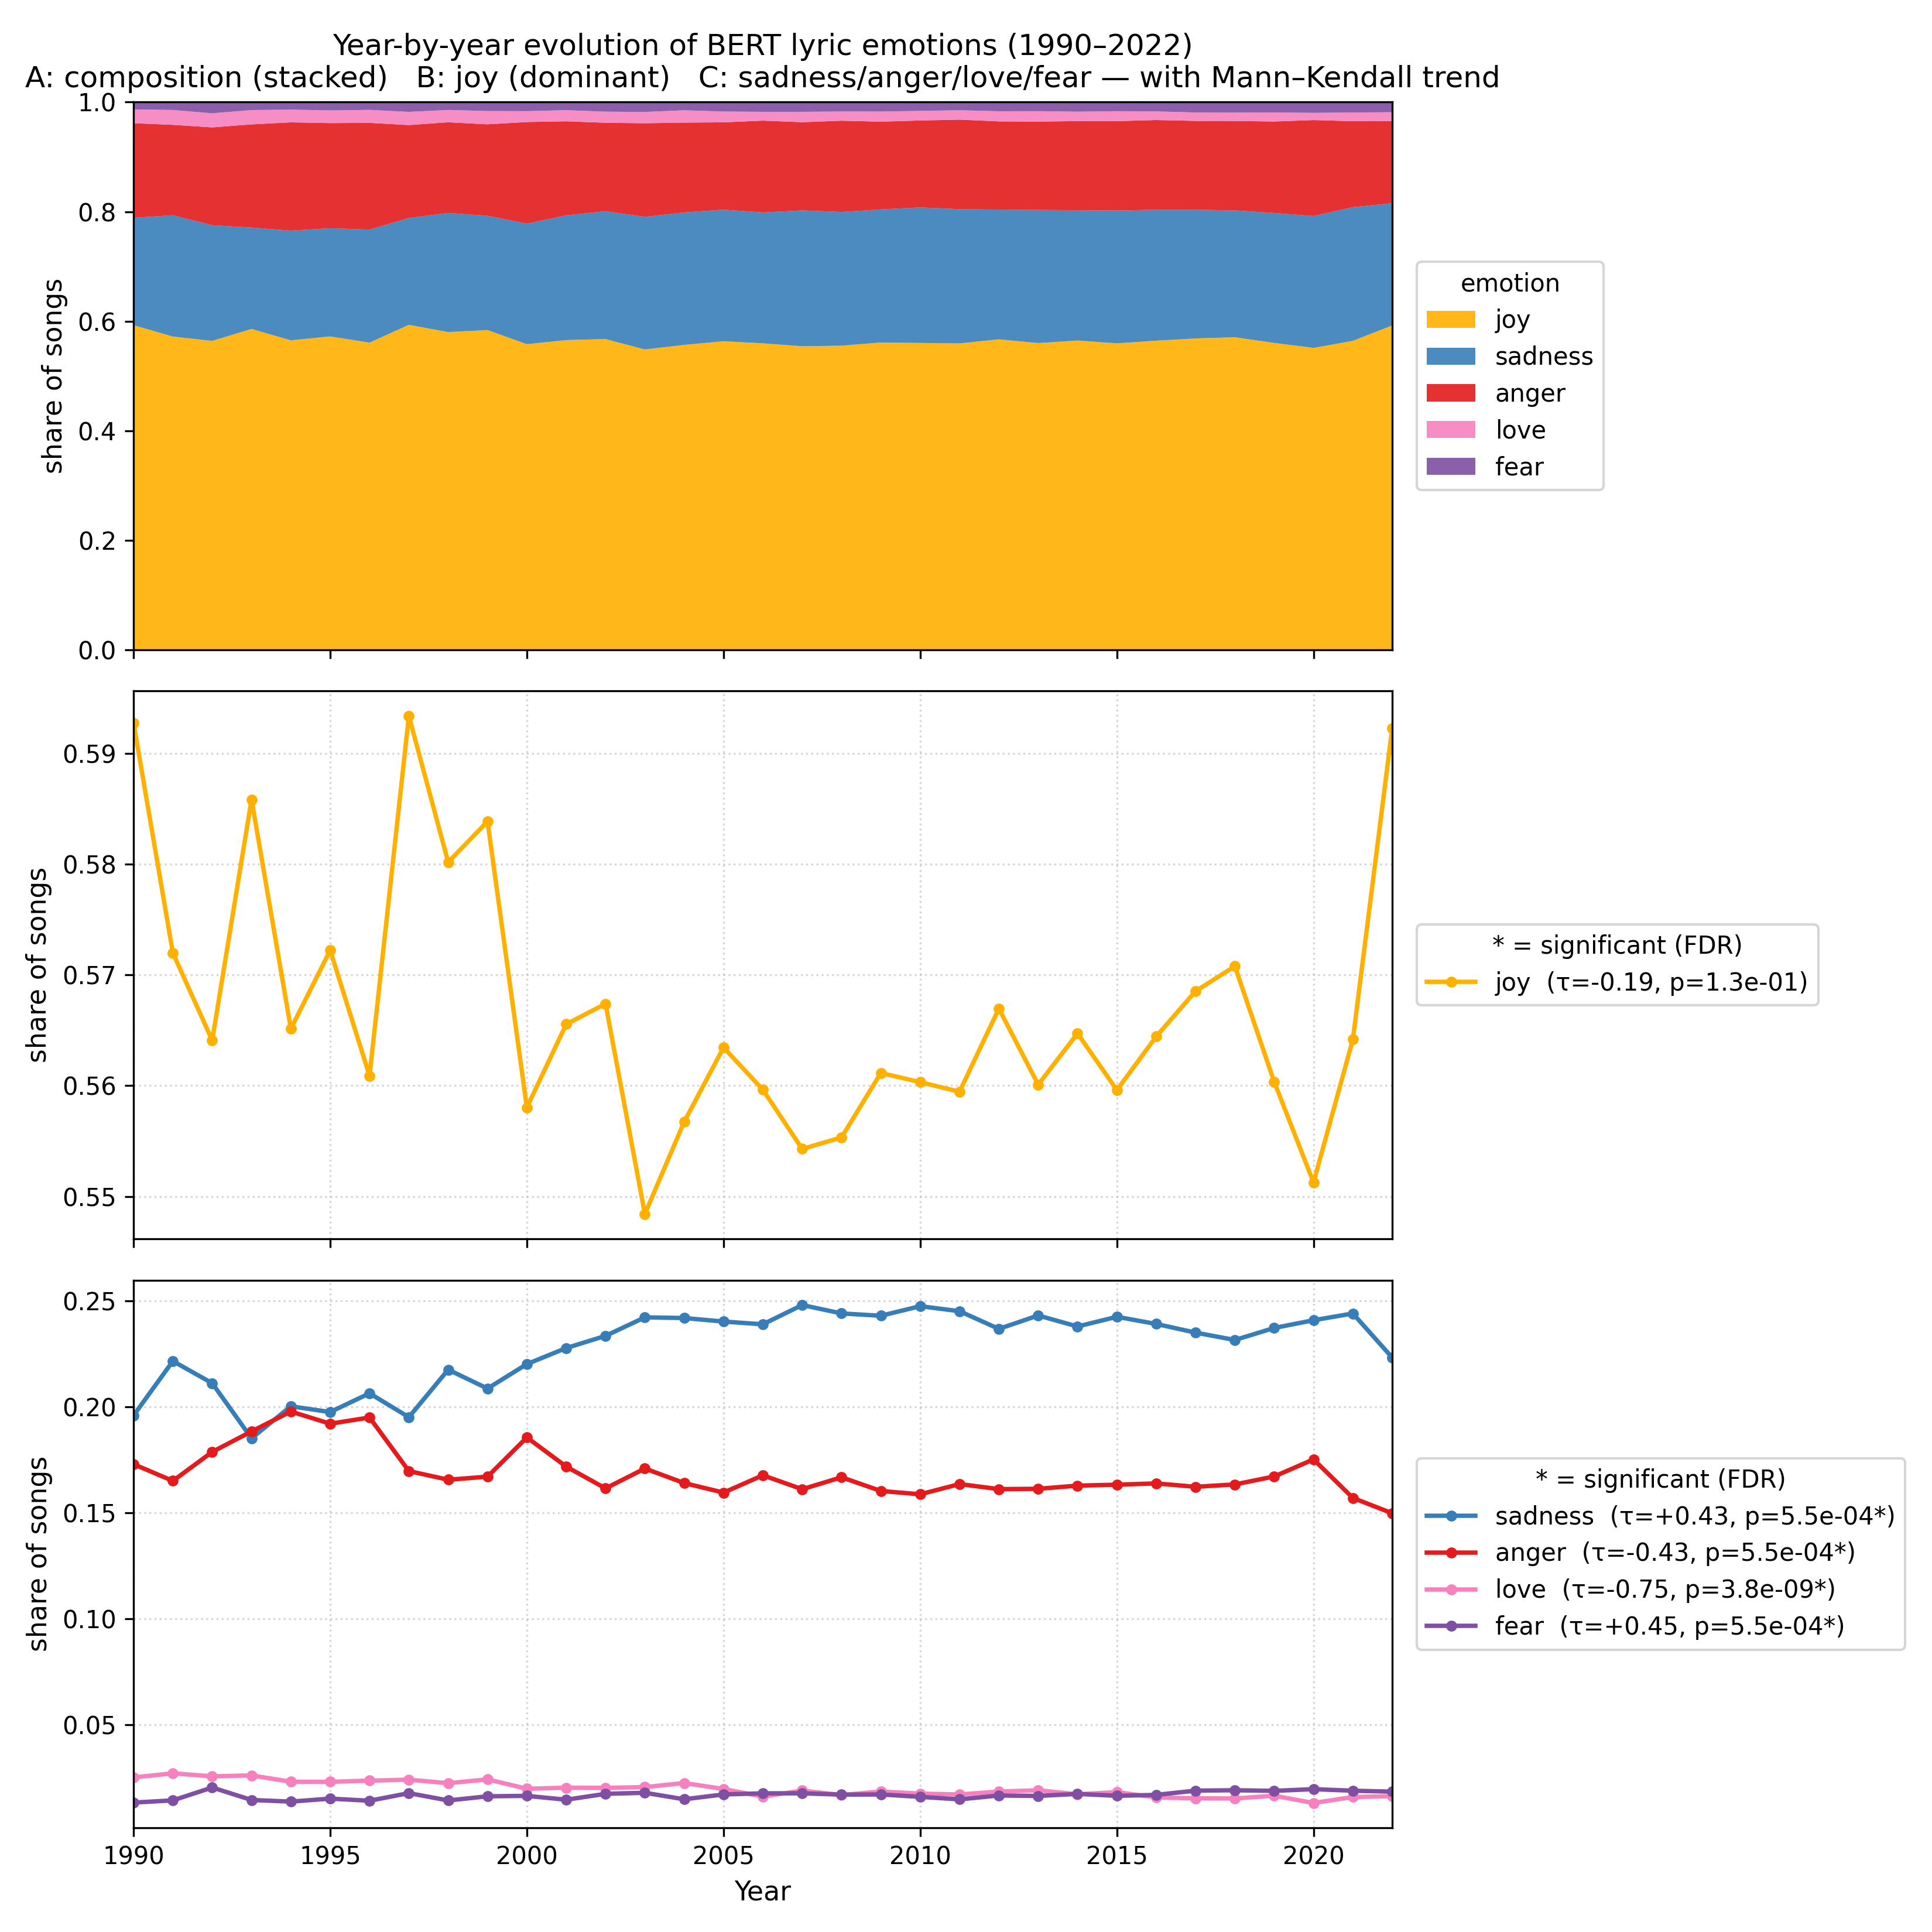
\includegraphics[width=\columnwidth]{fig8_emotion_trends.png}}
\caption{Year-by-year evolution of the five BERT lyric emotions, 1990--2022.}
\label{fig:emotions}
\end{figure}

\begin{figure}[htbp]
\centerline{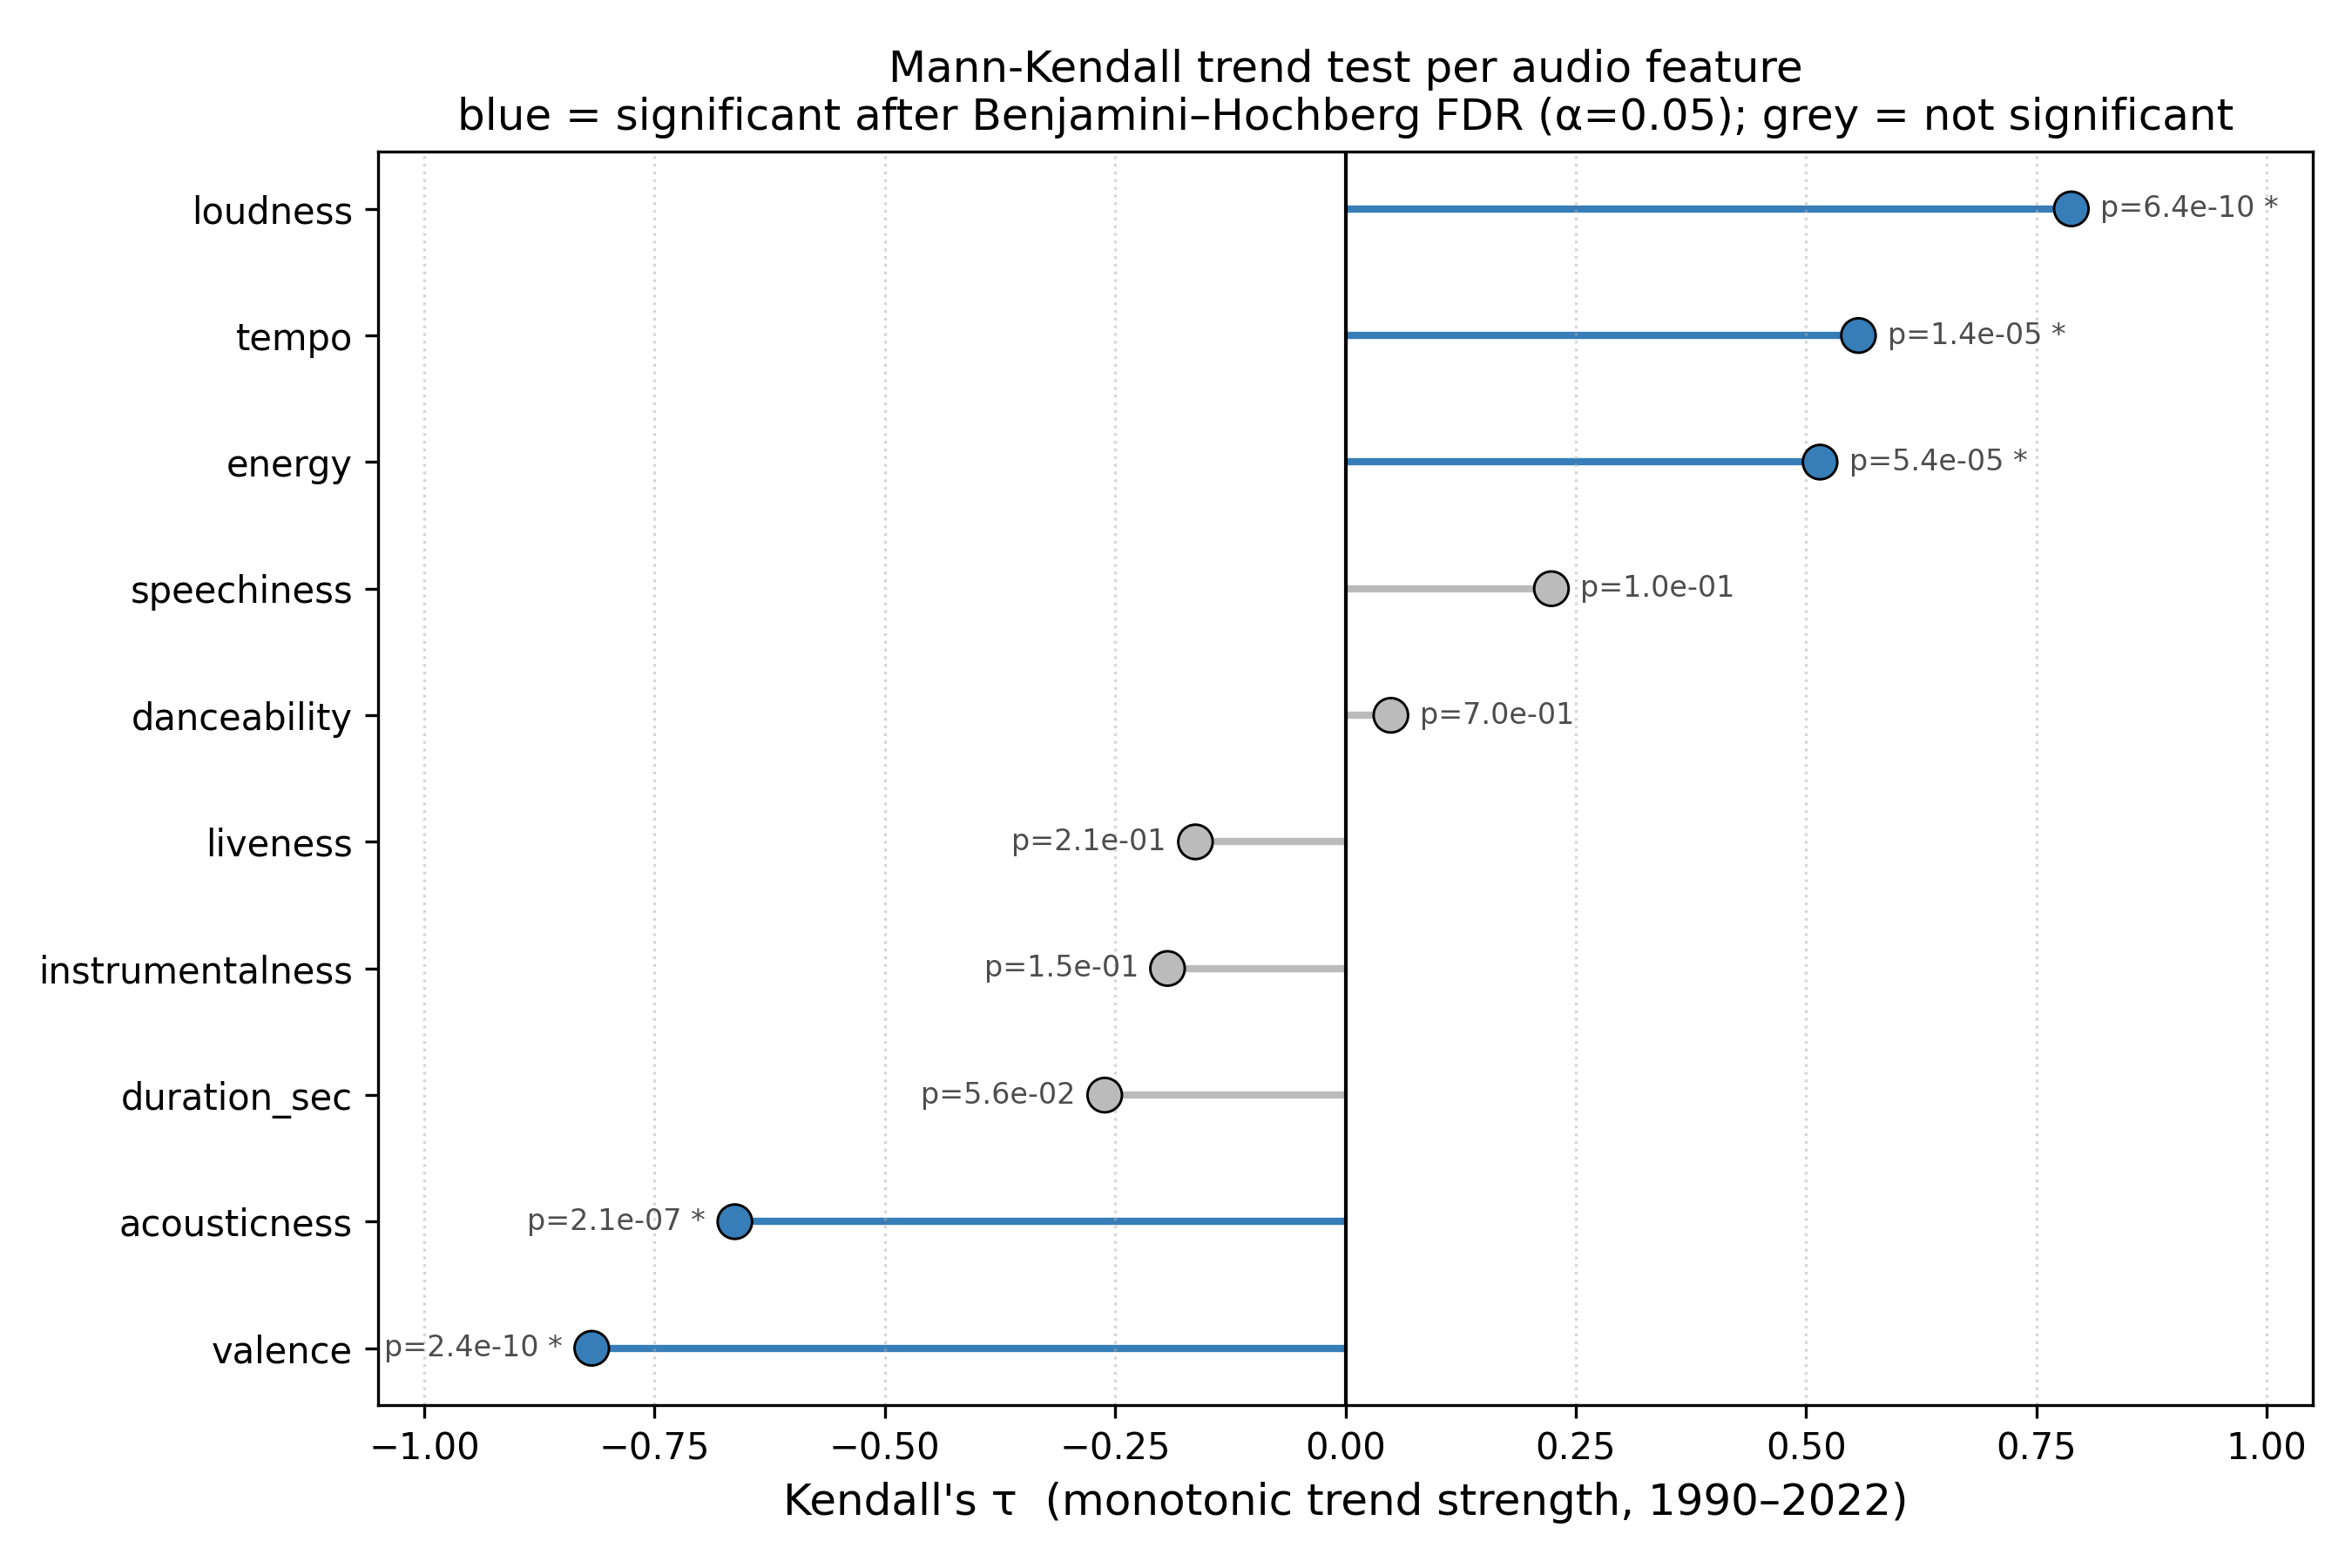
\includegraphics[width=\columnwidth]{fig5_feature_trend_tests.png}}
\caption{Mann--Kendall trend strength per audio feature.}
\label{fig:tau}
\end{figure}

\begin{figure}[htbp]
\centerline{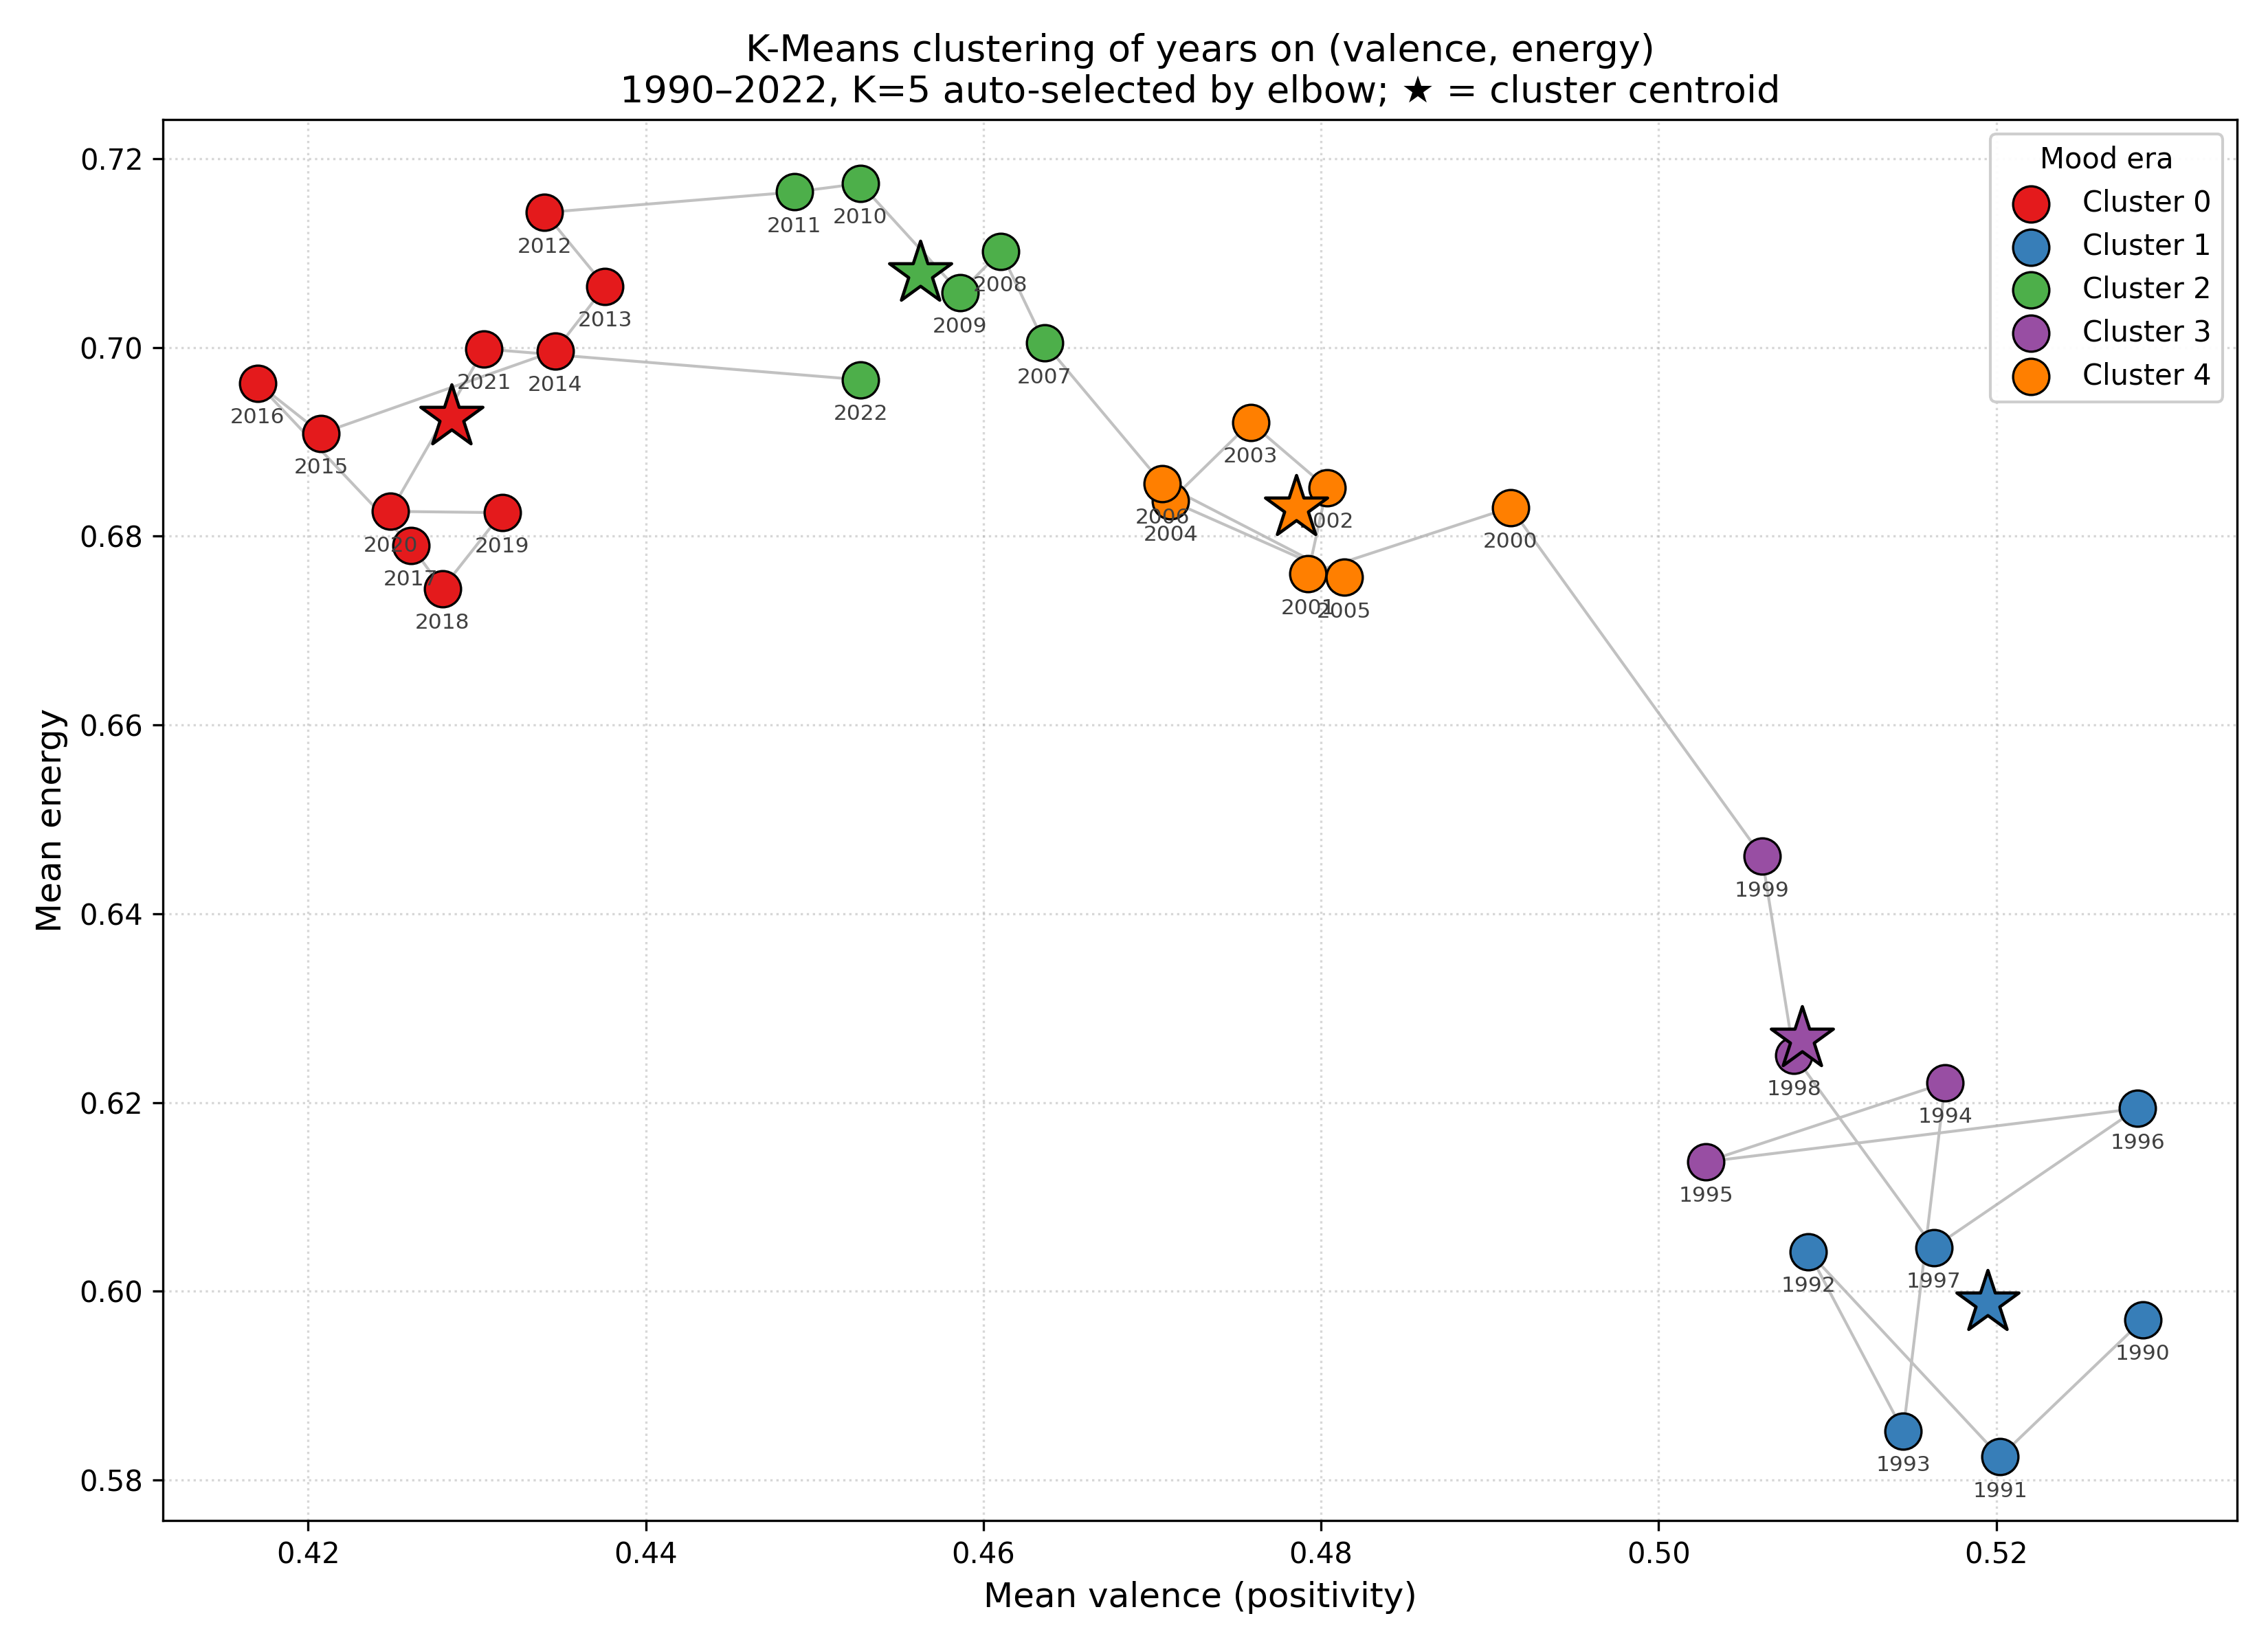
\includegraphics[width=\columnwidth]{fig1_mood_scatter.png}}
\caption{K-Means clustering of years on (valence, energy).}
\label{fig:mood}
\end{figure}

% Double-column (full width) figure -- good for the consensus raster:
\begin{figure*}[htbp]
\centerline{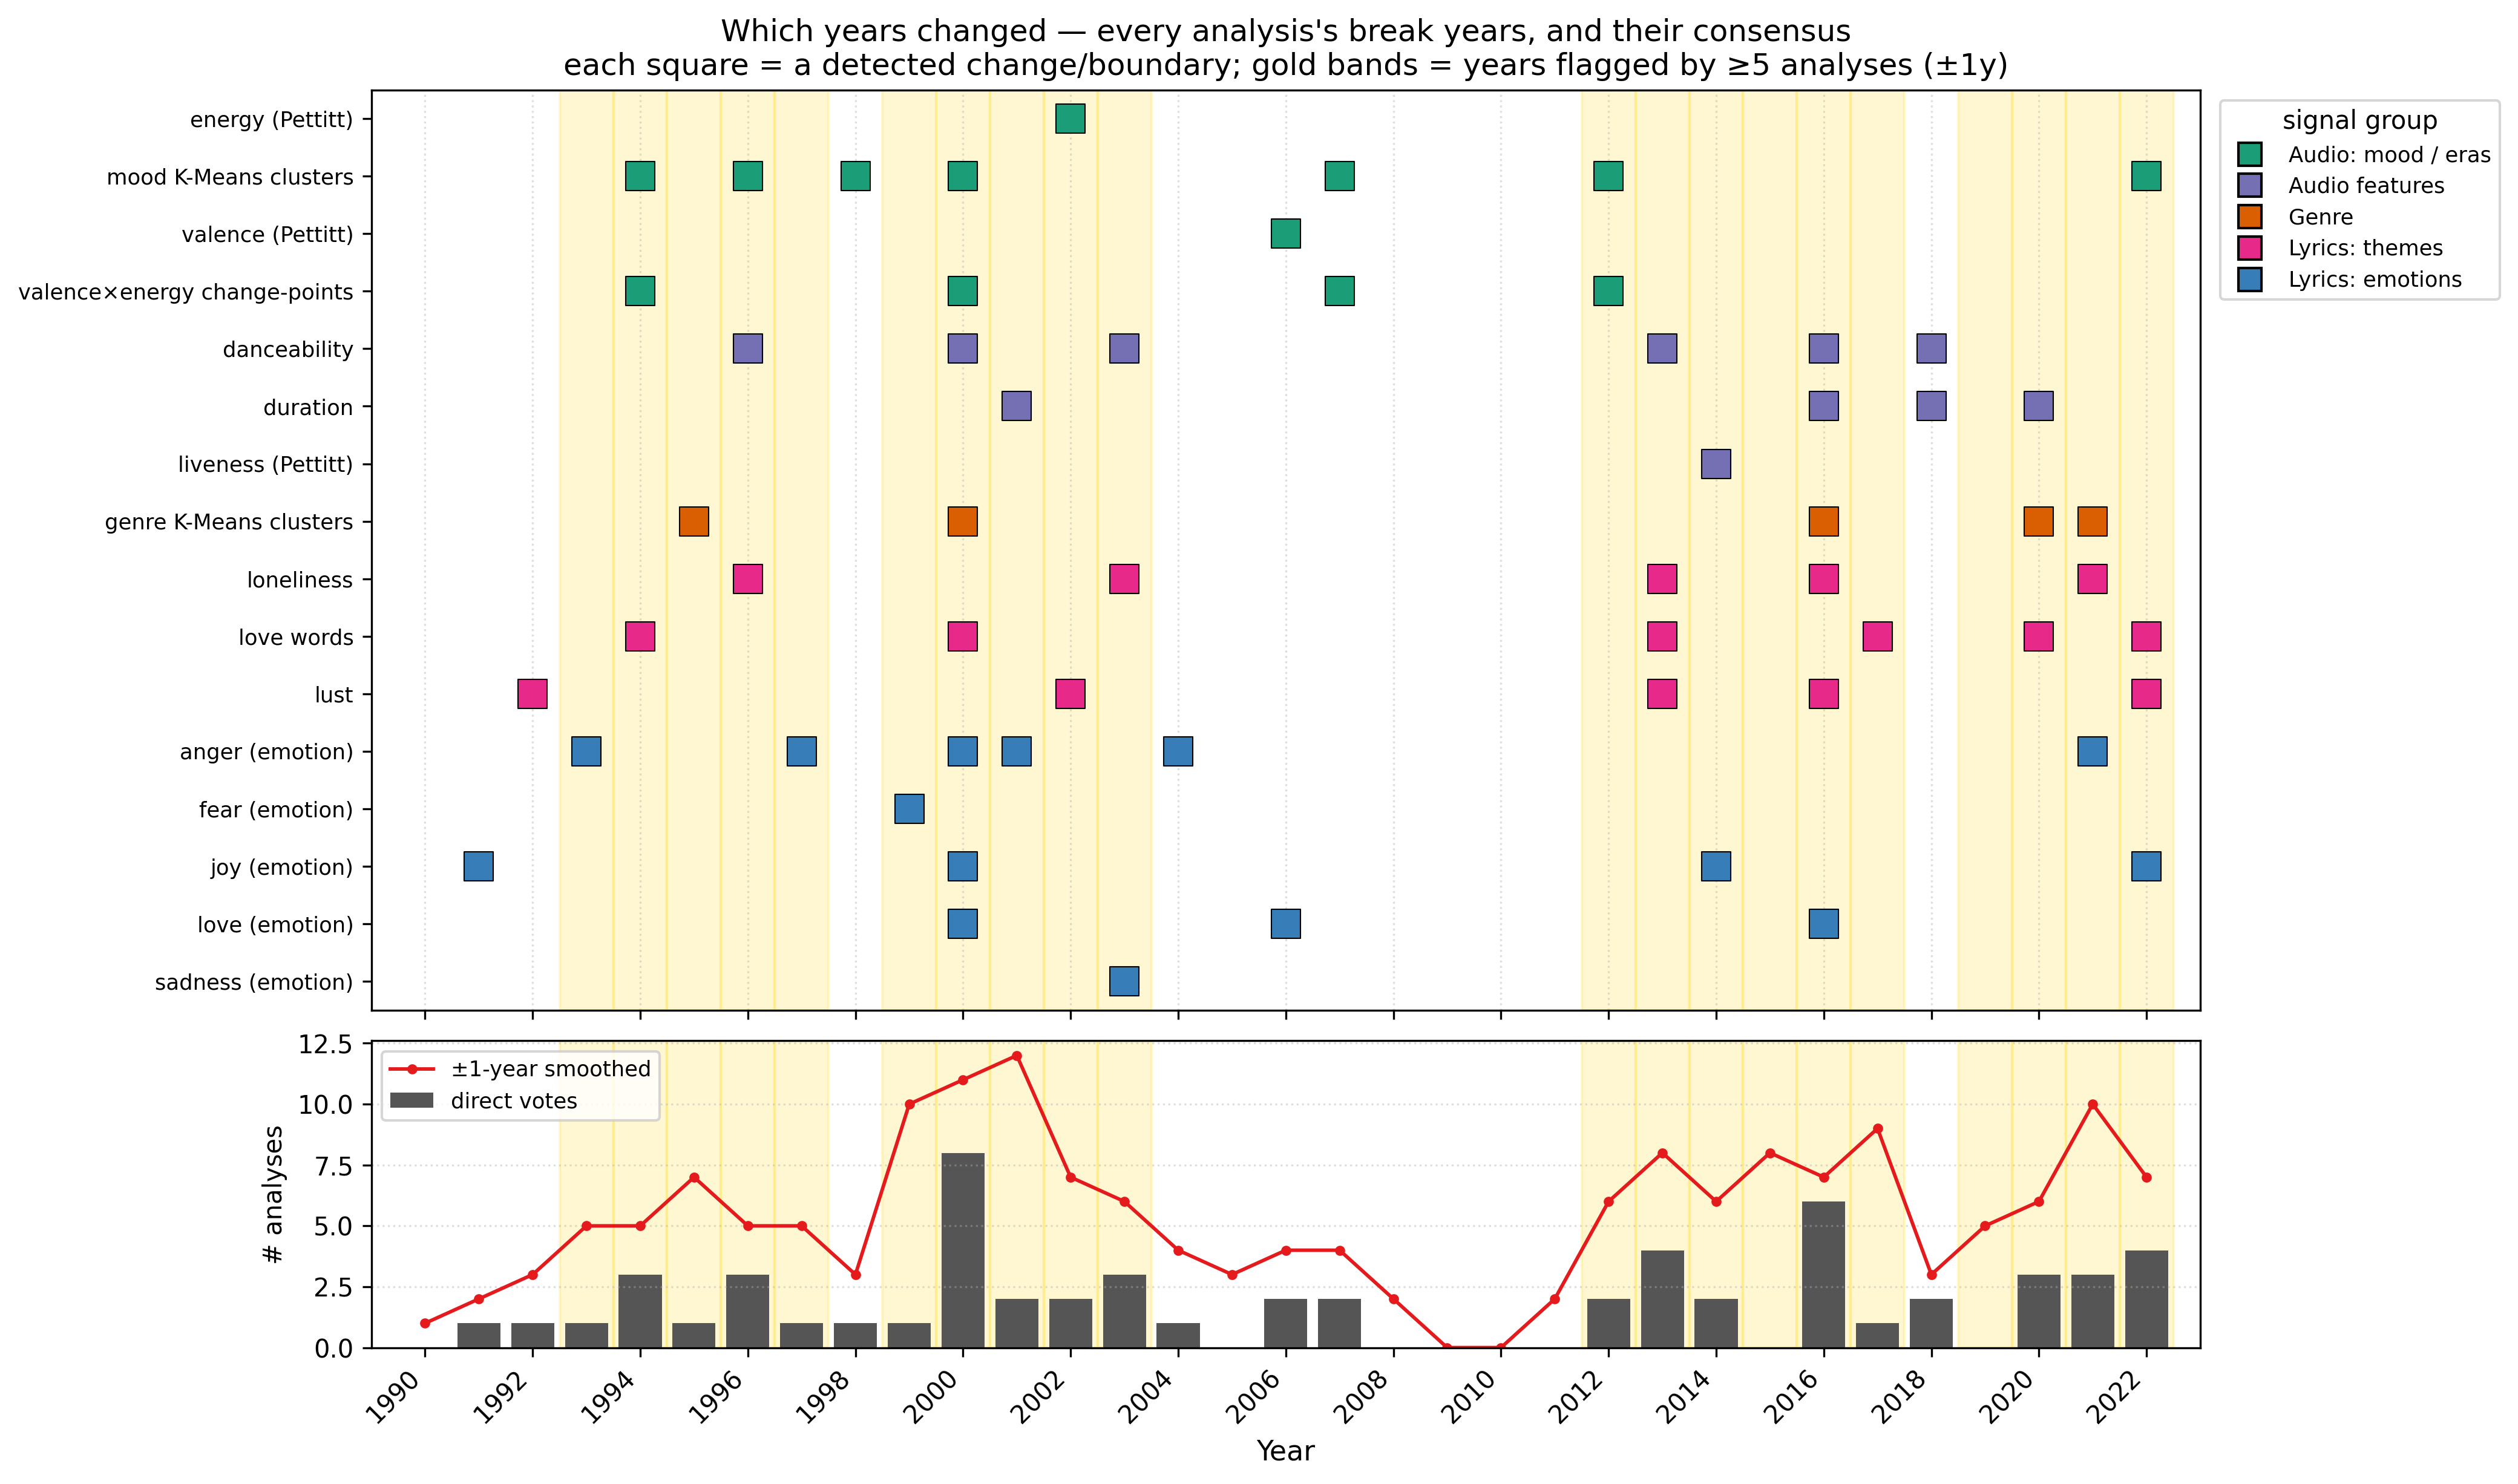
\includegraphics[width=\textwidth]{fig9_change_synthesis.png}}
\caption{Consensus of detected change years across every analysis.}
\label{fig:synthesis}
\end{figure*}

\begin{figure}[htbp]
\centerline{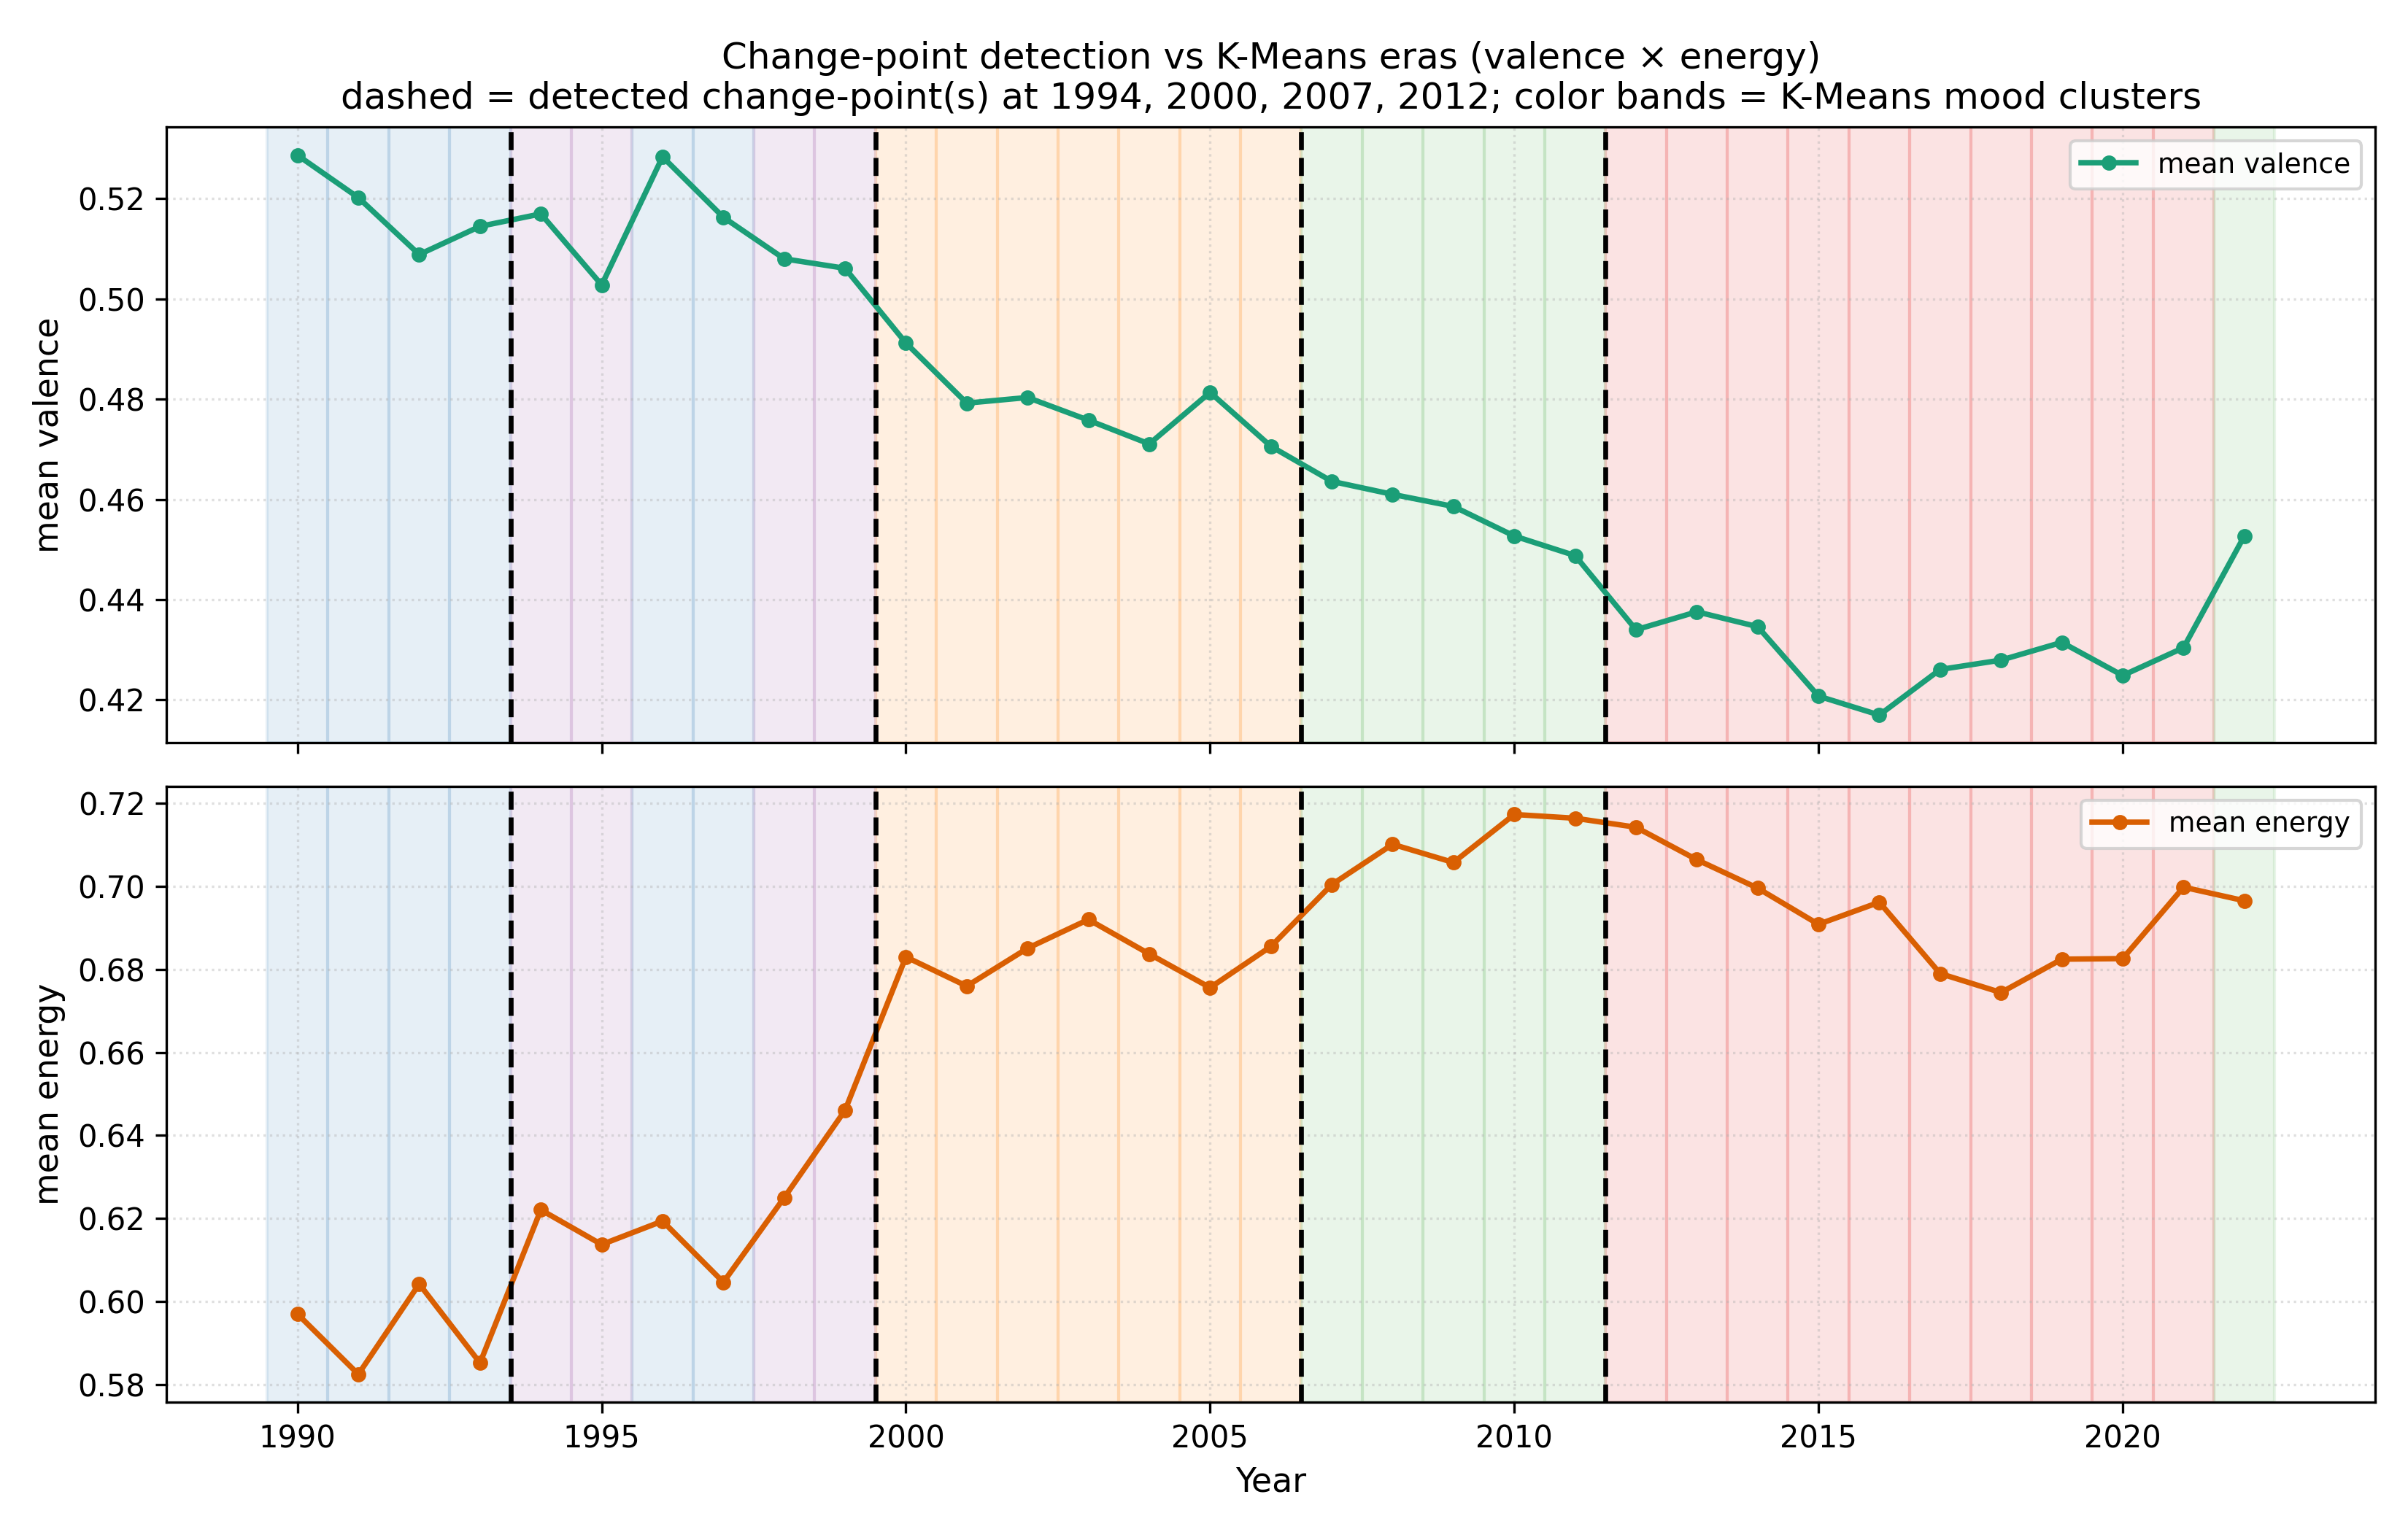
\includegraphics[width=\columnwidth]{fig6_change_points.png}}
\caption{Mean valence and energy over time with BIC-selected change-points
(dashed) and K-Means mood-cluster bands (background).}
\label{fig:changepoints}
\end{figure}

% Results table placeholder:
\begin{table}[htbp]
\caption{Mann--Kendall Trend Tests per Audio Feature, 1990--2022. Asterisks
Mark Trends Significant After Benjamini--Hochberg FDR Correction
($\alpha = 0.05$).}
\begin{center}
\begin{tabular}{|l|c|c|c|}
\hline
\textbf{Feature} & \textbf{Kendall} $\boldsymbol{\tau}$ & \textbf{$p$ (FDR)} & \textbf{Direction} \\
\hline
valence          & $-0.82$ & $2.4{\times}10^{-10}$ & decreasing$^{*}$ \\
loudness         & $+0.79$ & $6.4{\times}10^{-10}$ & increasing$^{*}$ \\
acousticness     & $-0.66$ & $2.1{\times}10^{-7}$  & decreasing$^{*}$ \\
tempo            & $+0.56$ & $1.4{\times}10^{-5}$  & increasing$^{*}$ \\
energy           & $+0.52$ & $5.4{\times}10^{-5}$  & increasing$^{*}$ \\
\hline
duration         & $-0.26$ & $0.056$ & decreasing \\
speechiness      & $+0.22$ & $0.100$ & increasing \\
instrumentalness & $-0.19$ & $0.147$ & decreasing \\
liveness         & $-0.16$ & $0.209$ & decreasing \\
danceability     & $+0.05$ & $0.698$ & increasing \\
\hline
\end{tabular}
\label{tab:trends}
\end{center}
\end{table}

\section{Discussion}

\subsection{Interpretation of the Observed Trends}
The two modalities tell a consistent story. Sonically, popular music became
louder, faster, more energetic, and less acoustic, yet steadily less positive in
valence---a combination best described as higher-arousal but lower-mood. The
lyric emotions move in the same direction: songs are progressively less often
dominated by love and more often by sadness and fear, even as joy remains the
most common single label. The low-valence, high-energy era that the clustering
isolates from roughly 2012 onward is therefore driven mainly by rising sadness
and fear rather than by anger, which in fact declines slightly across the full
period.

A salient short-term episode is the COVID-19 pandemic. Around 2020 the lyric
emotions shift: love reaches its lowest share of the entire study window while
anger spikes and fear stays elevated, and the loneliness vocabulary rises in the
same window. Mean valence also dips in 2020 and then recovers to one of its
highest values of the late period by 2022, consistent with a temporary
emotional downturn around the lockdowns followed by a rebound as they ended.
We stress that these are \emph{correlations} in time, not causal claims: our
design observes that musical mood and the pandemic coincide, but it cannot
establish that one caused the other.

\subsection{Convergent Validity Across Methods}
The central turning point near the year 2000 is not the product of any single
estimator. Unsupervised K-Means cluster boundaries, exact BIC change-points on
(valence, energy), Pettitt's significance-tested breaks, per-feature
change-points, and the change-points of the BERT emotion shares all place a
boundary at or within a year of 2000 (Fig.~\ref{fig:synthesis}). Because these
methods rest on different assumptions, their agreement is strong evidence that
2000 marks a genuine structural shift rather than a methodological artifact. The
one productive disagreement is between the BERT love share, which falls, and the
lexical love-word density, which is U-shaped and ends higher than it began: the
transformer measures how often love is a song's \emph{dominant} emotional
framing, whereas the lexicon measures raw mention frequency, and the two need
not move together.

\subsection{Threats to Validity and Limitations}
Several caveats bound these conclusions. First, the corpus is a catalogue
sample, not a listening- or popularity-weighted sample of what audiences
actually heard; trends describe the music that was \emph{released}, not its
reception. Second, the corpus grows roughly tenfold over the period, with a
sharp jump near 2000 that coincides with our dominant turning point; per-year
normalization removes the size effect from levels, but the coincidence warrants
caution in over-interpreting the exact year. Third, the emotion classifier is a
BERT model trained on general affective text rather than song lyrics, and may
misread figurative or repetitive lyrical language; the dominant-emotion rule
also discards within-song nuance. Fourth, the audio features are Spotify's
proprietary estimates, and the lyrics are English-centric. Finally, and most
importantly, every relationship reported here is correlational: we document that
musical mood changed over time and that some shifts coincide with external
events, but we make no causal claim.

\section{Conclusion and Future Work}
Across 489{,}761 songs spanning 1990 to 2022, popular music grew measurably
louder, more energetic, and less acoustic while becoming less positive in
valence, and its lyrics grew less love-dominated and more sad and fearful
(answering RQ1 and RQ2). Unsupervised clustering and statistical change-point
detection independently recover discrete eras and converge on a dominant turning
point around the year 2000 (RQ3). Future work could weight the corpus by
popularity or streaming counts to capture reception rather than release,
fine-tune the emotion classifier on lyrics, extend the analysis to non-English
repertoires, and relate the observed turning points to external cultural and
technological events---such as the rise of streaming and social media, or the
COVID-19 pandemic---in a framework able to test those associations explicitly.

\begin{thebibliography}{00}
\bibitem{b_dataset} serkantysz, ``550K+ Spotify Songs (Audio, Lyrics, and Genres),'' Kaggle, 2024. [Online]. Available: \url{https://www.kaggle.com/datasets/serkantysz/550k-spotify-songs-audio-lyrics-and-genres}
\bibitem{b_spark} M. Zaharia \textit{et al.}, ``Apache Spark: a unified engine for big data processing,'' \textit{Commun. ACM}, vol. 59, no. 11, pp. 56--65, 2016.
\bibitem{b_sparknlp} V. Kocaman and D. Talby, ``Spark NLP: natural language understanding at scale,'' \textit{Software Impacts}, vol. 8, art. 100058, 2021.
\bibitem{b_bert} J. Devlin, M.-W. Chang, K. Lee, and K. Toutanova, ``BERT: pre-training of deep bidirectional transformers for language understanding,'' in \textit{Proc. NAACL-HLT}, 2019, pp. 4171--4186.
\bibitem{b_emotion} E. Saravia, H.-C. T. Liu, Y.-H. Huang, J. Wu, and Y.-S. Chen, ``CARER: contextualized affect representations for emotion recognition,'' in \textit{Proc. EMNLP}, 2018, pp. 3687--3697.
\bibitem{b_mk} H. B. Mann, ``Nonparametric tests against trend,'' \textit{Econometrica}, vol. 13, no. 3, pp. 245--259, 1945.
\bibitem{b_sen} P. K. Sen, ``Estimates of the regression coefficient based on Kendall's tau,'' \textit{J. Amer. Statist. Assoc.}, vol. 63, no. 324, pp. 1379--1389, 1968.
\bibitem{b_bh} Y. Benjamini and Y. Hochberg, ``Controlling the false discovery rate: a practical and powerful approach to multiple testing,'' \textit{J. Roy. Statist. Soc. B}, vol. 57, no. 1, pp. 289--300, 1995.
\bibitem{b_pettitt} A. N. Pettitt, ``A non-parametric approach to the change-point problem,'' \textit{J. Roy. Statist. Soc. C}, vol. 28, no. 2, pp. 126--135, 1979.
\bibitem{b_bic} N. R. Zhang and D. O. Siegmund, ``A modified Bayes information criterion with applications to the analysis of comparative genomic hybridization data,'' \textit{Biometrics}, vol. 63, no. 1, pp. 22--32, 2007.
\bibitem{b_kneedle} V. Satopaa, J. Albrecht, D. Irwin, and B. Raghavan, ``Finding a `kneedle' in a haystack: detecting knee points in system behavior,'' in \textit{Proc. 31st IEEE ICDCS Workshops}, 2011, pp. 166--171.
\end{thebibliography}

\end{document}
